\subsection{Trích xuất và biểu diễn đặc trưng}

Dưới góc nhìn một bài toán truy xuất ảnh, các đặc trưng biểu diễn của ảnh sẽ mang tính quyết định đối với chất lượng và hiệu năng của cả mô hình. Để đảm bảo khả năng biểu diễn tốt cho các đặc trưng ảnh ở các địa danh khác nhau, quá trình trích xuất đặc trưng, ban đầu, được thiết kế một cách thủ công, đến từ kiến thức chuyên môn. Các nghiên cứu bước đầu đặt ra các định nghĩa về các loại đặc trưng: đặc trưng lân cận, đặc trưng toàn cục và độ quan trọng của chúng. Thời gian gần đây, với sự phát triển của thị giác máy tính, các phương pháp học biểu diễn bằng mạng nơ-ron học sâu đạt được các thành tựu nổi bật, đặc biệt là mạng nơ-ron tích chập thay thế chức năng của đặc trưng thủ công.

\subsubsection{Biễu diễn đặc trưng lân cận - Local descriptors}

Trong bài toán học biễu diễn đặc trưng, một đặc trưng lân cận chỉ phân tích, biểu diễn ý nghĩa của một nhóm các điểm ảnh nhỏ và chỉ ra sự khác biệt giữa chúng với các nhóm các điểm ảnh lân cận \cite{CGV-017-localdescriptors}. Các nhóm điểm ảnh được tạo ra bằng cách chia mỗi hình ảnh thành lưới với độ phân giải nhất định và tất cả các nhóm điểm ảnh được thu thập, trích xuất để tìm đặc trưng. Để áp dụng cho bài toán truy xuất hình ảnh trực quan, các thuật toán lựa chọn như Hessian-Affine detector \cite{hessian-affine-detector}, MSER\cite{MSER-detector} được áp dụng để lựa chọn chỉ những nhóm điểm ảnh mang tính quan trọng, quyết định đến sự khác nhau giữa các ảnh và loại bỏ các nhóm điểm ảnh dễ bị ảnh hưởng bởi yếu tố môi trường. Vào thời gian đầu, việc truy xuất đặc trưng từ các nhóm ảnh, điểm ảnh được thực hiện bằng cách sử dụng các thuật toán như SIFT \cite{lowe1999object}, SURF \cite{bay2006surf}, RootSIFT \cite{Arandjelovi2012ThreeTE}, BRIEF \cite{brief}, DSP-SIFT \cite{Dong2014DomainsizePI} và đặc trưng kernel \cite{kernel-descriptors}. Các hướng tiếp cận mới hơn cho rằng các hướng tiếp cận trên sử dụng số lượng lớn đặc trưng cần trích xuất và lưu trữ trong khi không phải tất cả các đặc trưng đều có đủ tính phân biệt cho quá trình truy xuất ảnh \cite{predicting-good-features}, từ đó, đề xuất thêm quá trình lọc đặc trưng vào quá trình trích xuất. Năm 2014, Jégou và Zisserman chuẩn hóa quá trình trích xuất véc-tơ biểu diễn từ đặc trưng cục bộ thành quy trình 2 bước\cite{Jegou_2014_CVPR}:
\begin{enumerate}
    \item bước nhúng chuyển mỗi véc-tơ đặc trưng lên không gian mới có số chiều cao hơn,
    \item bước tổng hợp tạo chỉ một véc-tơ biểu diễn từ các véc-tơ đã tạo.
\end{enumerate}
Năm 2015, \cite{selective-match-kernel} đề xuất hàng loạt các phương án cho các bước nhúng, tổng hợp, cùng với các giải pháp để lựa chọn mức độ đóng góp của mỗi cặp biểu diễn cho một nhóm các ảnh, đánh dấu nền móng về hướng phát triển và hiện thực cho các mô hình học biễu diễn đặc trưng cục bộ sau này.

\subsubsection{Biễu diễn đặc trưng toàn cục  - Global descriptors}

Trong khi việc tổng hợp các véc-tơ biểu diễn cục bộ hỗ trợ việc truy xuất một véc-tơ biễu diễn cho một hình ảnh, các véc-tơ biểu diễn toàn cục có thể truy xuất tất cả thông tin này một cách trực tiếp. Khác với véc-tơ trích xuất cục bộ, các véc-tơ trích xuất toàn cục đọc và trích xuất biểu diễn đặc trưng cho toàn bộ bức ảnh và chỉ ra các đặc điểm khác biệt giữa bức ảnh này và bức ảnh khác. Việc truy xuất véc-tơ toàn cục có thể được hiện thực và thực thi với yêu cầu tài nguyên ít hơn sơ với việc truy xuất véc-tơ cục bộ, nhưng đồng thời cũng giảm đi khả năng phân biệt và tính bền bỉ trước các yếu tố thay đổi do điều kiện môi trường, góc chụp và các yếu tố bị che khuất. Mặc dù vậy, lợi ích của việc trích xuất đặc trưng cục bộ, áp dụng bởi các phương pháp như HOG \cite{HOG}, Gist \cite{GIST}, vẫn được xem trọng trong quá trình trích xuất biểu diễn đặc trưng toàn cục và trở thành cảm hứng cho các mô hình học biểu diễn sử dụng mạng nơ-ron học sâu sau này.

\subsubsection{Học biễu diễn bằng mạng nơ-ron học sâu tích chập và các lớp kết nối đầy đủ}

Với sự thành công của mạng nơ-ron học sâu trong lĩnh vực thị giác máy tính\cite{krizhevsky2012imagenet}, các mô hình học sâu này đã được công nhận là những phương pháp tạo biểu diễn vô cùng hiệu quả. Đồng thời, một số bài báo cũng đã chỉ ra khả năng học đặc trưng thường thấy và chuyển tiếp được (transferable) đến các bài toán khác \cite{Oquab_2014_CVPR,ZeilerVisualizingAU,Chen2018DeepLabSI}.

\begin{figure}[h]
    \centering
    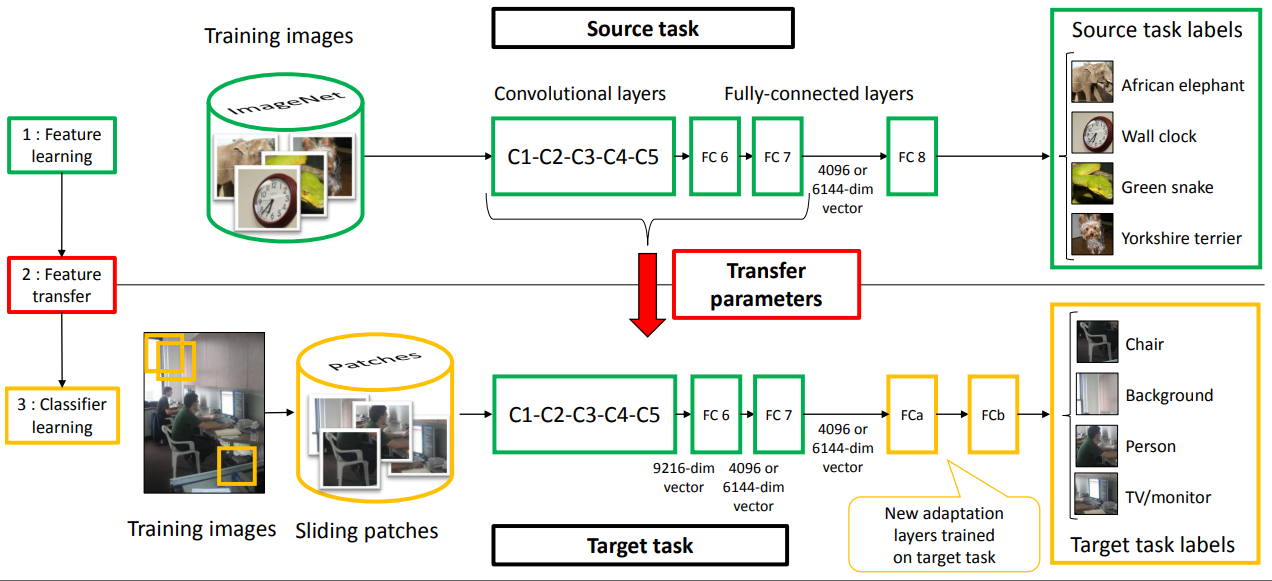
\includegraphics[width=\textwidth]{pics/Chapter2/cnn_transfer.png}
    \caption{Chuyển tiếp thông số của một mô hình mạng nơ-ron học sâu tích chập\cite{Oquab_2014_CVPR}}
\end{figure}

Các mô hình học sâu tích chập đầu tiên được sử dụng cho bài toán truy xuất hình ảnh trực quan được cấu hình từ các lớp kết nối đầy đủ\cite{razavian2014cnn, gong2014multiscale, babenko2014neural, deepindex, image-classification-retrieval, wang2014deep} của một mạng phân loại, được huấn luyện trên tập dữ liệu ImageNet\cite{russakovsky2015imagenet}, đạt hiệu quả đáng kể khi sử dụng hàm mất mát triplet\cite{wang2014deep, gomezojeda2015training}. Tuy nhiên, có thể sớm nhận thấy rằng các mô hình sử dụng nhiều lớp kết nối đầy đủ có ý nghĩa tương ứng với các biểu diễn đặc trưng toàn cục. Các biểu diễn đặc trưng tạo ra được bằng cách sử dụng phương pháp này thiếu độ bền đối với dữ liệu chứa nhiều yếu tố gây nhiễu, che khuất và không đủ các yếu tố bất biến đối với biến thể tịnh tiến và tỉ lệ. Để khắc phục các hạn chế này, nhiều mô hình học sâu đã đề xuất các phương án cắt ảnh thành nhiều nhóm điểm ảnh và huấn luyện nhiều biểu diễn với kết nối đầy đủ cho mỗi hình \cite{razavian2014cnn, babenko2014neural}. Khi đánh giá các cách tiếp cận này so với các phương pháp trích xuất đặc trưng thủ công cục bộ, các mô hình học sâu sử dụng ít bộ nhớ hơn nhưng yêu cầu số lượng tính toán cao hơn. Các biểu diễn kết nối đầy đủ bị giới hạn bởi kích thước đầu vào cố định và lượng lớn các tham số.

\subsubsection{Học biểu diễn bằng mạng nơ-ron tích chập}

Nỗ lực tìm giải pháp cho các giới hạn của mạng nơ-ron kết nối đầy đủ đã trở thành cảm hứng cho các phương pháp sử dụng trực tiếp kết quả nhận được từ các lớp tích chập của mạng nơ-ron học sâu. Áp dụng hướng tiếp cận đầu tiên chính là bài nghiên cứu của Babenko và nnk \cite{babenko2014neural}. Mạng nơ-ron tích chập tạo ra một tenxơ (tensor) có cấu hình \(H \times W \times C\), trong đó \(C\) là số kênh, \(H\) và \(W\) là chiều cao và chiều rộng của ảnh. Babenko và nnk tạo ra véc-tơ biểu diễn bằng cách làm phẳng và chuẩn hóa lớp \(H \times W \times C\). Một số bài báo lấy cảm hứng từ hướng nghiên cứu này \cite{hou2015convolutional}, sau đó, đã thể hiện rằng véc-tơ biểu diễn mạng nơ-ron học được, tùy vào phương án kết hợp lớp tenxơ, có thể mang ý nghĩa và chức năng tương tự với biểu diễn đặc trưng toàn cục trong khi tránh được các hạn chế của các mô hình học sâu sử dụng lớp kết nối đầy đủ. Các giải pháp này có thể được phân loại vào hai nhóm chính \cite{Masone2021ASO}:

\begin{itemize}
    \item gom cụm đặc trưng (feature aggregation) tích chập bằng các giải pháp lấy cảm hứng từ trích xuất đặc trưng thủ công cục bộ;
    \item tổng hợp đặc trưng (feature pooling) bằng cách khái quát hóa các đặc trưng tích chập.
\end{itemize}

\begin{figure}[h]
    \centering
    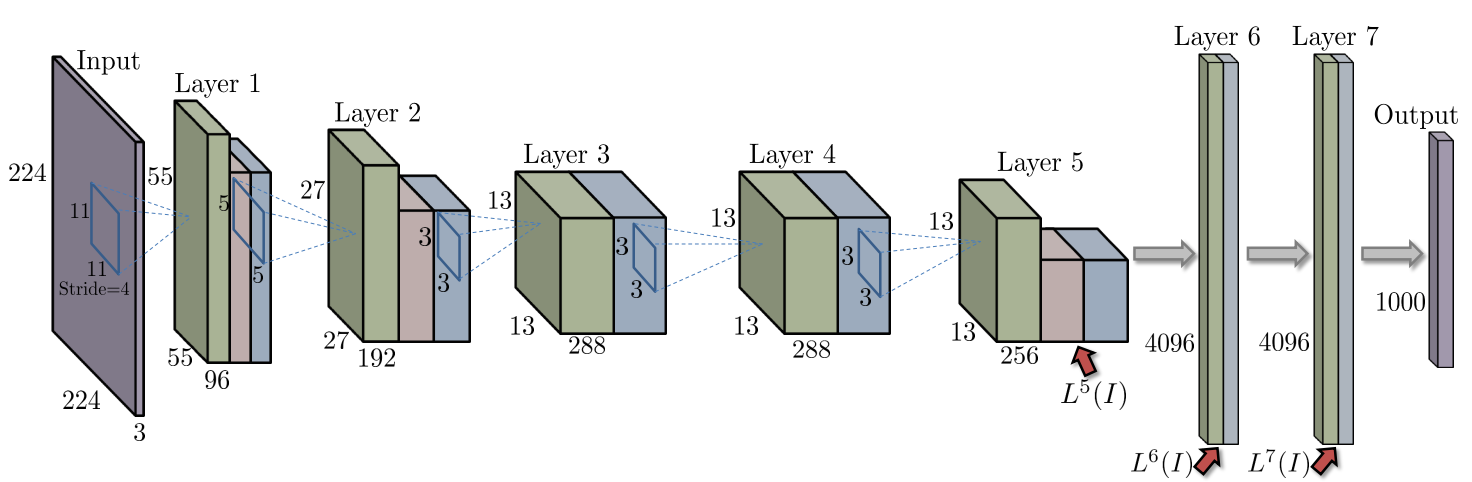
\includegraphics[width=\textwidth]{pics/Chapter2/firstcnns.png}
    \caption{Minh họa kiến trúc một mô hình CNN \cite{babenko2014neural}}
\end{figure}

Khi thực hiện gom đặc trưng trên lớp đặc trưng \(H \times W \times C\), lớp tích chập được đặt dưới góc nhìn là một lưới \(H \times W \) chứa các đặc trưng \(C\) chiều với mỗi đặc trưng là một véc-tơ có vùng nhận thức nhỏ. Bằng cách này, kết quả nhận được từ lớp tích chập có thể được đồng hóa (assimilated) thành một tập hợp các véc-tơ cục bộ được bố trí dày đặc. Tập hợp các véc-tơ dày đặc tiếp tục được mã hóa thành một véc-tơ biểu diễn và được sử dụng cho quá trình so sánh và truy xuất bằng các giải thuật so sánh tương đồng như khoảng cách Euclidean, tương đồng cosine. Sử dụng phương pháp này, việc mã hóa đặc trưng cho bước tìm kiếm tương đồng có thể áp dụng các hướng tiếp cận xử lý đặc trưng thủ công cục bộ như VLAD\cite{vlad}, BoW\cite{Mohedano_2016}, ASMK\cite{cao2020unifying}. Các nhà nghiên cứu tiếp tục đề xuất các phương pháp gom cụm có khả năng kết hợp trực tiếp với mạng nơ-ron tích chập toàn bộ để cung cấp khả năng huấn luyện cả mô hình đầu-cuối \cite{ong2017siamese}. Đánh dấu một bước tiến quan trọng trong nỗ lực tìm giải pháp cho bài toán nhận diện địa điểm trực quan chính là lớp gom cụm NetVLAD \cite{arandjelovic2016netvlad}, hiện thực mô hình mã hóa và gom cụm VLAD với các phép tính khả vi cho phép mô hình khả năng huấn luyện đầu cuối một cách linh hoạt với nhiều tham số huấn luyện hơn so với VLAD thông thường. Hướng tiếp cận của các tác giả NetVLAD được tiếp tục hiện thực và sử dụng đến nay, đồng thời trở thành cảm hứng cho các hướng tiếp cận hiện đại hơn sau này.

\begin{figure}[h]
    \centering
    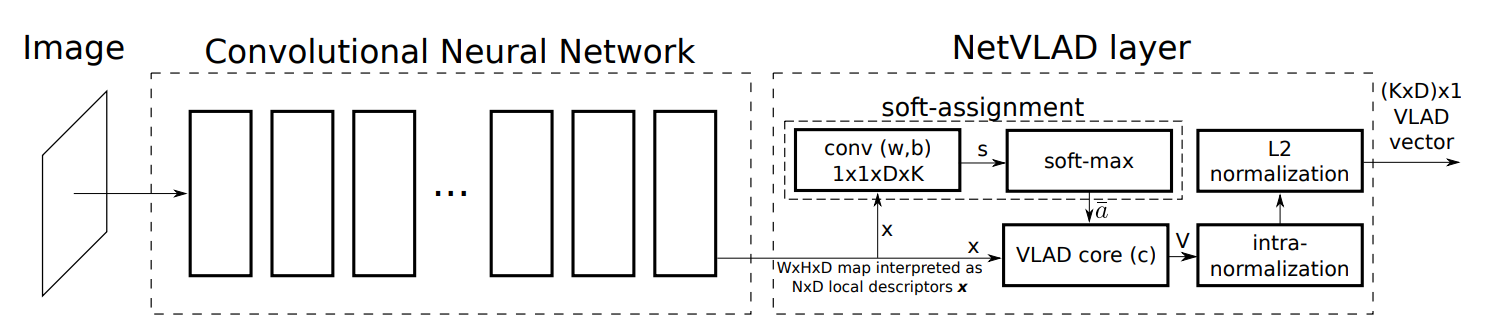
\includegraphics[width=\textwidth]{pics/Chapter2/netvladcnn.png}
    \caption{Minh họa kiến trúc một mô hình CNN được kết nối với lớp NetVLAD \cite{arandjelovic2016netvlad}}
\end{figure}

Tổng hợp đặc trưng lấy cảm hứng từ các nghiên cứu về mạng nơ-ron tích chập. Các nhà nghiên cứu đã chỉ ra các đặc trưng từ những lớp tích chập giữa, cuối có tiềm năng được gom đặc trưng và sử dụng trực tiếp cho quá trình phân loại và tìm kiếm tương qua mà không cần mã hóa. Quá trình tổng hợp đặc trưng, tuy có thể được thực hiện một cách tương đối đơn giản như việc sử dụng một lớp max-pooling, lại truy xuất được các đặc trưng biểu diễn với số chiều thấp, mức chiếm dụng bộ nhớ thấp và hiệu năng vượt trội hơn so với đặc trưng biểu diễn được thiết kế thủ công. Các tác giả của bài báo \cite{mousavian2015deep} nhận thấy rằng phương pháp max-pooling có độ bền cao hơn đối với sự thay đổi về tỉ lệ trong khi sum-pooling có độ nhạy với các yếu tố gây nhiễu hơn. Họ kiểm thử một mô hình kết hợp cả hai phương pháp, SPoC, với mục đích đúc kết được điểm mạnh của cả hai phương pháp và đã đạt kết quả đáng kể. Tương tự, Tolias và những cộng sự \cite{tolias2015particular} phát triển quy trình mã hóa R-MAC (Regional Maximum Activations of Convolutions), tính toán véc-tơ max-pooling cho nhiều vùng ảnh khác nhau và tổng hợp chúng bằng lớp sum-pooling. R-MAC và SPoC là cảm hứng cho sự ra đời của GeM \cite{GeM} - lớp aggregation trung bình tổng quát. Áp dụng một tham số cho mỗi lớp đặc trưng và hiện thực lớp trung bình tổng quát dự trên các tham số đó, GeM đạt được hiệu quả vượt trội hơn cả R-MAC và SPoC và trở thành một trong những phương pháp tổng hợp đặc trưng hiệu quả nhất cho đến nay.